\documentclass[../main.tex]{subfiles}

\begin{document}

\chapter{Methodology}
The methodology used in this project:
\begin{itemize}
    \item Theory studies.
    \begin{itemize}
        \item Graph theory.
        \item Maps and routing.
    \end{itemize}
    \item Analysis.
    \begin{itemize}
        \item Tools.
        \item Design.
    \end{itemize}
    \item Development (incremental).
    \begin{itemize}
        \item Coding.
        \item Testing.
        \item Documenting.
    \end{itemize}
    \item Evaluation.
\end{itemize}

\noindent
The \textit{``Detailed problem statement''} in section \ref{sect:detailed-problem} and the final specifications in appendix \ref{appendix-specification} resolves some of these steps: several of the tools are given, while the investigation for the others are described below. 

The methodology to use for the development is also given, either \emph{Behaviour Driven Development, BDD} or \emph{Test Driven Development, TDD}, meaning all features of the module have either a \emph{scenario} (BDD) or a \emph{test case} (TDD) written. This is suitable to use with an incremental, iterative development model, where one is constantly re-evaluating and adding and testing new features. One could move the ``design'' step from ``Analysis'' and under ``Development'' as the design is allowed to change. The \textit{coding standard} gives guidance on \textit{coding} and \textit{documentation}. 

Another part of testing, is visual examination to see that the graphs looks like expected. There will also be performance tests, to see that the software fulfills the requirements for \textit{soft real-time} execution. There will also be evaluation of fulfillment of the other requirements in the specification.

\vspace{1em}
\noindent
As for tools, some are given in the specifications (see Appendix \ref{appendix-specification}), while others have been chosen during a selection process. Below is presented the tools chosen, and in some cases what alternatives that were also considered and tested. The categories are:

\begin{itemize}
    \item Behaviour and Test Driven Development.
    \item Database.
    \begin{itemize}
        \item Database and extensions.
        \item Loading OpenStreetMap into database.
        \item Build topology.
        \item Examining map data.
        \item Connecting to database from application.
    \end{itemize}
    \item Reading configurations from \texttt{json}-file.
    \item Building graph.
\end{itemize}


%=====================================================================================
\section{Behaviour and Test Driven Development}
\emph{Behaviour Driven Development} tests usually have the structure: 
$Scenario \rightarrow Given \rightarrow When \rightarrow Then$, written with words to describe the steps. An example in the \emph{Gherkin} language is shown in listing \ref{lst:gherkin-example}.

\begin{mylisting}
\begin{gherkincode}
Scenario: vectors can be sized and resized
     Given: A vector with some items
     When:  the size is increased
     Then:  the size and capacity change
\end{gherkincode}
\caption{Example of a BDD scenario in \emph{Gherkin}.}
\label{lst:gherkin-example}
\end{mylisting}

So when developing BDD style one has to think through different scenarios and write them down, which can be helpful when thinking about what one tries to accomplish.

%.....................................................................................
\subsection{Tools, installation and usage}\label{catch-tool}
The testing library for this project is \href{http://www.catch-lib.net}{Catch}\footnote{\url{http://www.catch-lib.net}}, which is a small library for both BDD and TDD, where the BDD \emph{``scenario''} corresponds to a TDD \emph{``test-case''}, and \emph{``given'', ``when'', ``then''} corresponds to \emph{``section''}, meaning one can choose the development style one wishes. \emph{Catch} was chosen because it is header only, and there is no need for complicated building of libraries and setting up paths; one can just include the header in the project and go.

Simply download the file \texttt{catch.hpp} and put it either in your project tree or in your path for includes.

Include the header in the source for your test, and get Catch to provide a \texttt{main}-method. See listing \ref{lst:bdd-catch} for an example of how to implement the above stated ``feature''.

\begin{mylisting}
\begin{cppcode}
#define CATCH_CONFIG_MAIN
#include "catch.hpp"
#include <vector>

SCENARIO ("Vectors can be sized and resized", "[vector]") {
	GIVEN ("A vector with some items") {
		std::vector<int> v(5);

		REQUIRE (v.size() == 5);
		REQUIRE (v.capacity() >= 5);

		WHEN ("the size is increased") {
			v.resize(10);

			THEN ("the size and capacity change") {
				REQUIRE (v.size() == 10);
				REQUIRE (v.capacity() >= 10);
			}
		}
	}
}
\end{cppcode}
\caption{A basic BDD scenario with Catch}
\label{lst:bdd-catch}
\end{mylisting}

%.....................................................................................
\subsection{Alternatives}
The BDD style of developing seems not to have caught on in c++ so much. There are a few libraries. \href{https://github.com/cucumber/cucumber-cpp}{Cucumber-Cpp}\footnote{\url{https://github.com/cucumber/cucumber-cpp}} was investigated as it is an implementation for c++ of the Cucumber tool, which is widespread in many programming languages, so one could write the test for features in the ordinary \texttt{.feature}-files in the \emph{Gherkin} language, that are common for writing features for tests. But I could not get Cucumber-Cpp to build correctly with CMake and the dependencies.

%.....................................................................................
\subsection{Remarks}
It should not be a very difficult task to write a script that reads a \texttt{.feature}-file and outputs a template in c++, using the Catch syntax.

If one were to \emph{not} go for BDD-style of testing, then one could go for TDD testing using Boost Test, if one would want to keep using Boost for most parts of the project.


%=====================================================================================
\section{Database}
The database of choice, and in the requirements of the project, is  \href{http://www.postgresql.org/}{PostgreSQL}\footnote{\url{http://www.postgresql.org/}}, with the extension \href{http://postgis.net/}{PostGIS}\footnote{\url{http://postgis.net/}} which gives the database \emph{spatial} and \emph{geographic} capabilities, which are needed to simplify working with maps and such, for example when needing to measure distances in different projections. How to set up the database with users and passwords and such are not given in this report, but it is not so hard. When setting up databases one can interact via either the commandline or a \emph{graphical user interface, GUI} such as \emph{pgAdmin3}.

%.....................................................................................
\subsection{Tools, installation and usage}
The tool set was given in the requirements, as mentioned before. On my Debian/Ubuntu system they can be installed as shown in listing \ref{lst:install-dbtools}.


\begin{mylisting}
\begin{bashcode}
$ sudo apt-get install postgresql postgresql-contrib-9.3 postgis postgresql-9.3-postgis-2.1 pgadmin3 osm2pgsql
\end{bashcode}
\caption{Installation of database tools}
\label{lst:install-dbtools}
\end{mylisting}

%.....................................................................................
Listing \ref{lst:setup-db} shows how to create a new database called \texttt{mikh\_db} with a user ``jonas'' (that is already set up as a user with rights to create databases), and enabling the needed spatial extensions to work with map data.

\begin{mylisting}
\begin{bashcode}
$ createdb mikh_db -U jonas
$ psql -U jonas -d mikh_db -c "CREATE extension postgis;"
$ psql -U jonas -d mikh_db -c "CREATE extension postgis_topology;"
$ psql -U jonas -d mikh_db -c "CREATE extension hstore;"
$ psql -U jonas -d mikh_db -c "SET search_path=topology, public;"
\end{bashcode}
\caption{Create database and enable spatial extensions.}
\label{lst:setup-db}
\end{mylisting}

%.....................................................................................
\subsection{Loading map data}
To get the \texttt{.osm}-file, which is actually in \texttt{xml}, into the database one needs a conversion tool to parse the file and populate some tables with data. 

%.....................................................................................
\subsubsection{Tools, installation and usage}
There exists several tools for importing \texttt{OSM} data into a database. It was hard to know which one to pick and different options were tried, but the chosen tool is \href{http://wiki.openstreetmap.org/wiki/Osm2pgsql}{osm2pgsql}\footnote{\url{http://wiki.openstreetmap.org/wiki/Osm2pgsql}}. It was installed in listing \ref{lst:install-dbtools}. 

\begin{mylisting}
\begin{bashcode}
$ osm2pgsql -U jonas -d mikh_db -k -s mikhailovsk.osm
\end{bashcode}
\caption{Usage of \texttt{osm2pgsql}.}
\label{lst:osm2pgsql}
\end{mylisting}

Listing \ref{lst:osm2pgsql} reads an \texttt{.osm}-file in the current directory and populates the database \texttt{mikh\_db}. The flags \texttt{-k} tells to use ``hstore'' for tags and, \texttt{-s} to make a ``slim'' conversion. Two different \texttt{.osm}-files have been provided for testing, ``mikhailovsk.osm'' and ``partille.osm'', hence the usage of ``mikhailovsk.osm''. 

One might specify other flags as well. Among the options is to chose a different projection than the default \texttt{900913}. It is also possible to specify a \texttt{.style}-file which is a configuration over which tags to import. It is possible to use this file to decide which tags to import into the database and which tags to discard.

\subsubsection{Alternatives}
There exists a bunch of other tools that can convert OpenStreetMap files into database tables, such as \emph{Osmosis, Imposm, osm2po, osm2pgrouting}, and others; all with different strengths and weaknesses, such as being good and free, but not open source.

%.....................................................................................
\subsection{Building topology}
With the data in the database, it is time to build a topology of the map data, saying how the vertices and edges are connected, to make it possible to build a routable graph. A lot of the ``nodes'' in the \texttt{osm}-data are only useful for describing the geometry, while what is interesting when routing are the nodes that connects edges; that is the junctions at which roads meet. Therefore it is essential to analyze the data an build tables that contain information about the topology.

One can have different thoughts of when to do this. It would be possible to do this at the preliminary step when loading the data into the database. That would be good if one was certain of that the topology is stable. If the network is more volatile, it would be better to build the topology on every query, to be certain that one always has the most up-to-date information. On the other hand; the topology for a road network should be stable, and temporary closures  and other changing conditions will be better reflected in tags that can be queried when calculating costs for routing. That is the path taken in this project.

\subsubsection{Tools, installation and usage}
The choice for this project is PostGIS' topology extension. It is a part of PostGIS, which is already installed.

The \texttt{osm}-data from \texttt{osm2pgsql} has a table for all the lines in the map, called \texttt{planet\_osm\_line}, but in addition to roads it contains lines for railways, waterways, borders, buildings etc. So to build routing data we need to extract the lines only representing the roads, and put it in a new table. Listing \ref{lst:db-create-roads-table} shows that.

\begin{mylisting}
\begin{bashcode}
$ psql -U jonas -d mikh_db -c "CREATE TABLE roads AS SELECT * FROM planet_osm_line WHERE highway IS NOT NULL;"
\end{bashcode}
\caption{Creating a table with only roads in it.}
\label{lst:db-create-roads-table}
\end{mylisting}

Then one can build a topology of the roads, as shown in listing \ref{lst:db-pg-topology}. The first line creates a new schema called \texttt{roads\_topo} which will hold the topology data in the projection \texttt{900913} (the projection used when loading the database). The second line adds a column called \texttt{topo\_geom} to the table \texttt{roads} in the public schema. The third line connects that column with the newly built corresponding topology in the \texttt{roads\_topo} schema. The topology is built with a tolerance of 1.0 units. The unit for this projection is meters, so it means that if there are several nodes within 1.0 meters or a node within 1.0 meters from a road, they are joined. This can be essential to building a routable network. When running the validation tool in JOSM on the \texttt{mikhailovsk.osm}-file, it reported 16 suspect cases with nodes close but not connected, see figure \ref{fig:qgis-not-connected}.

\begin{mylisting}
\begin{bashcode}
$ psql -U jonas -d mikh_db -c "SELECT topology.CreateTopology('roads_topo', 900913);"
$ psql -U jonas -d mikh_db -c "SELECT topology.AddTopoGeometryColumn('roads_topo', 'public', 'roads', 'topo_geom', 'LINESTRING');"
$ psql -U jonas -d mikh_db -c "UPDATE roads SET topo_geom = topology.toTopoGeom(way, 'roads_topo', 1, 1.0);"
\end{bashcode}
\caption{Building a topology with PostGIS.}
\label{lst:db-pg-topology}
\end{mylisting}

\begin{figure}[h]
    \centering
    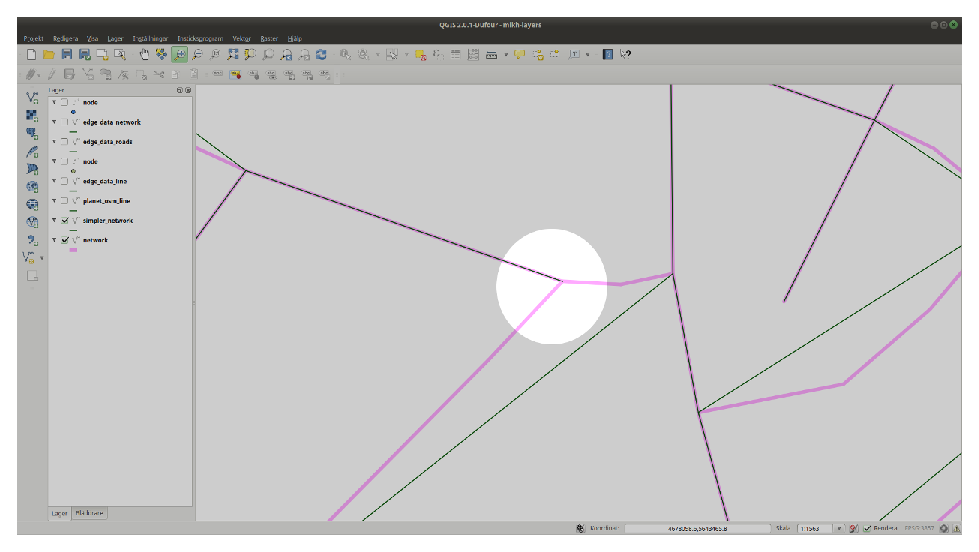
\includegraphics[width=0.9\linewidth]{qgis-not-connected-roads}
    \caption{Error building topology with a node close but not connected.}
    \label{fig:qgis-not-connected}
\end{figure}

\subsubsection{Alternatives}
One might load the database, and build a topology with \href{http://pgrouting.org/docs/tools/osm2pgrouting.html}{osm2pgrouting}\footnote{\url{http://pgrouting.org/docs/tools/osm2pgrouting.html}}, and the PostgreSQL extension \href{http://pgrouting.org/index.html}{pgRouting}\footnote{\url{http://pgrouting.org/index.html}}. That solution is pretty smooth, and might heal the topology with a tolerance, but it seems it only builds the topology and does not give access to tags and other information usable when calculating costs.

Another attempt, was to run a topology building SQL function (as in \url{http://blog.loudhush.ro/2011/10/using-pgrouting-on-osm-database.html}), and then run another function to remove all nodes without topological meaning. But that lead to the problem shown in figure \ref{fig:qgis-not-connected}, as there had been no ``healing'' of nodes first. One solution could of course to write another function for that, or to fix the \texttt{.osm}-file manually in JOSM before loading it into the database. But the solution with the PostGIS topology seems like a better way to go.

%.....................................................................................
\subsection{Examining map data}
Map data lends itself to visualization. And it is also useful to build a mental model of what one is working on, and to see the results.

\subsubsection{JOSM}
\href{https://josm.openstreetmap.de/}{JOSM}\footnote{\url{https://josm.openstreetmap.de/}} is an editor for OpenStreetMap. It can open \texttt{.osm}-files and display them, inspect elements of the map, and it has tools for editing and validation, meaning one might be able to fix files that has problems. See figure \ref{fig:josm-mikhailovsk}.

\begin{figure}[h]
    \centering
    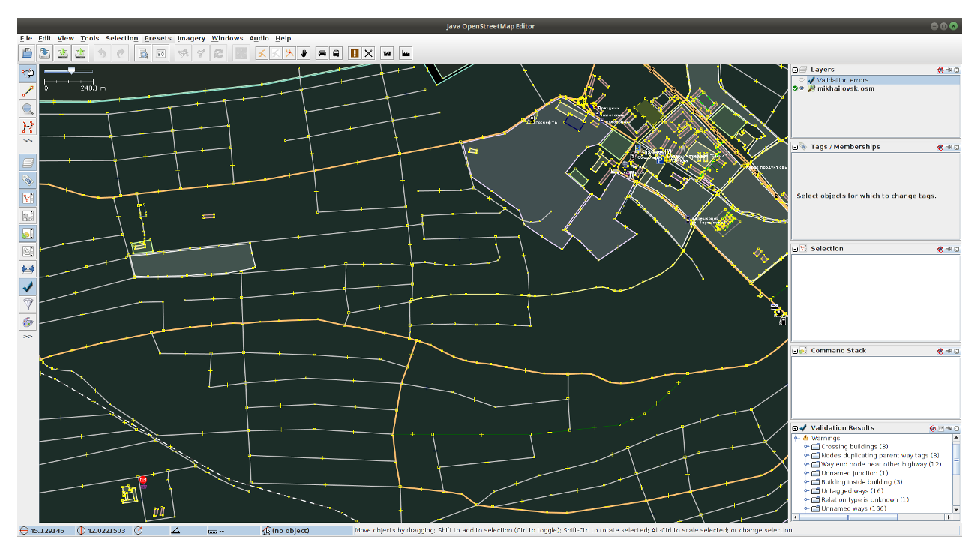
\includegraphics[width=0.9\linewidth]{josm-mikhailovsk}
    \caption{JOSM editor with Mikhailovsk map.}
    \label{fig:josm-mikhailovsk}
\end{figure}

\subsubsection{QGIS}
\href{http://www.qgis.org/}{QGIS}\footnote{\url{http://www.qgis.org/}} is a tool that can load spatial data from databases and display, as well as load for example \texttt{.osm}-files. It makes it good to visualize for example query results or transformations you have made in the database. See figure \ref{fig:qgis-mikhailovsk} for an example with layers of PostGIS-data of ``Mikhailovsk'' on top of each other.

\begin{figure}[h]
    \centering
    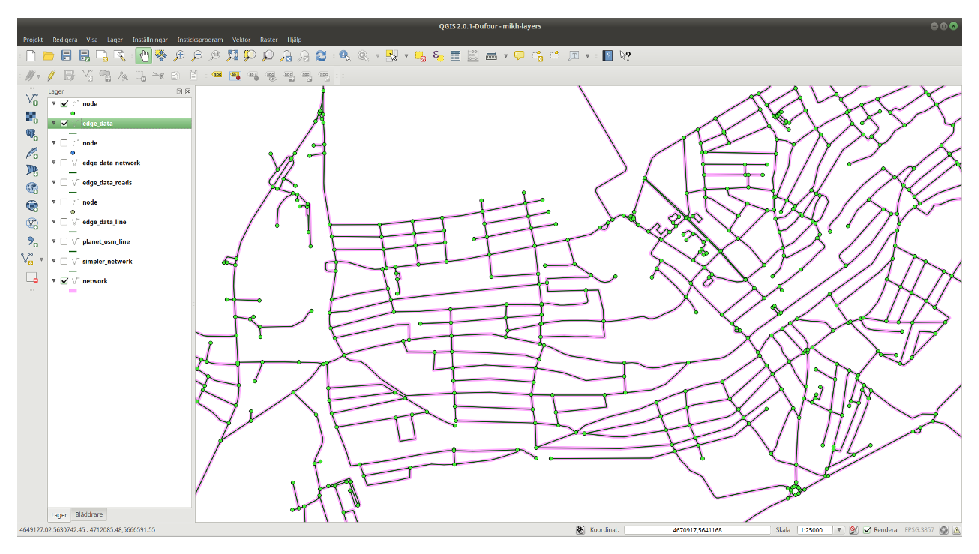
\includegraphics[width=0.9\linewidth]{qgis-pg_topology-highways-nodes}
    \caption{QGIS editor with Mikhailovsk map from PostGIS tables.}
    \label{fig:qgis-mikhailovsk}
\end{figure}

When loading data from PostGIS one might have to specify which projection to use for display. The default projection when loading \texttt{.osm}-files into the database using \texttt{osm2pgsql} is \texttt{SRID 900913}, and to display that correctly in QGIS one needs to use the projection \texttt{EPSG:3857}.

%=====================================================================================
%.....................................................................................
\subsection{Connecting to database}
After the module has read in the configuration, the next step is to connect to the database and perform some work on the map data before extracting relevant information.

The connection to the PostgreSQL database is handled by the library \href{http://pqxx.org/development/libpqxx/}{libpqxx}\footnote{\url{http://pqxx.org/development/libpqxx/}}, and while there exists a few alternatives, it is natural to go for the official alternative.

%.....................................................................................
\subsubsection{Tool, installation and usage}
Installation of \texttt{libpqxx} is shown in listing \ref{lst:libpqxx-installation}.

\begin{mylisting}
\begin{bashcode}
$ sudo apt-get install libpqxx-4.0
\end{bashcode}
\caption{Installing \texttt{libpqxx} on a Debian/Ubuntu system.}
\label{lst:libpqxx-installation}
\end{mylisting}

It is pretty straightforward to use: include the header, make connections and transactions. A snippet is shown in listing \ref{lst:libpqxx-connection}.

\begin{mylisting}
\begin{cppcode}
#include <pqxx/pqxx>
...
pqxx::connection conn("dbname=testdb user=tester password=tester hostaddr=127.0.0.1 port=5432");
\end{cppcode}
\caption{Include header and make a connection to the database.}
\label{lst:libpqxx-connection}
\end{mylisting}

When compiling, one must link with the libraries \texttt{pqxx} and \texttt{pq}, as shown in listing \ref{lst:libpqxx-link}.

\begin{mylisting}
\begin{bashcode}
$ g++ mytest.cpp -lpqxx -lpq -o mytest
\end{bashcode}
\caption{Linking \texttt{libpqxx} at compile time.}
\label{lst:libpqxx-link}
\end{mylisting}


%=====================================================================================
\section{Configuration}
The module should be configured by a settings file, written as \emph{json}. Settings can be related to the database such as host address, table names etc; or it can be configuration of costs for the routing such as speed limits, traffic lights, turn restrictions. 

%.....................................................................................
\subsection{Tools, installation and usage}
There is no meaning in writing a json-parser for this module as there exists lots of good libraries. The one chosen is \href{http://www.boost.org/doc/libs/1_54_0/doc/html/property_tree.html}{Boost Property Tree}\footnote{\url{http://www.boost.org/doc/libs/1_54_0/doc/html/property_tree.html}}, as the project uses other Boost libraries, and it simple enough to get started with.

As several Boost packages will be used in this project, it is just as good installing all of them (for a Debian/Ubuntu based system), see listing \ref{lst:boost-install}.

\begin{mylisting}
\begin{bashcode}
$ sudo apt-get install libboost-all-dev
\end{bashcode}
\caption{Installation of Boost libraries.}
\label{lst:boost-install}
\end{mylisting}

An example to see how simple it is to parse a json-file is shown in listing \ref{lst:boost-pt-example}.

\begin{mylisting}
\begin{cppcode}
#include <string>
#include <iostream>
#include <boost/property_tree/ptree.hpp>
#include <boost/property_tree/json_parser.hpp>

void readJsonFile(const std::string& filename) {
	boost::property_tree::ptree pt;
	boost::property_tree::read_json(filename, pt);
	std::string host = pt.get<std::string>("host");
	int port = pt.get<int>("port");
	std::cout << "Host: " << host << ", port: " << port << std::endl;
}
\end{cppcode}
\caption{Parsing a json-file.}
\label{lst:boost-pt-example}
\end{mylisting}


%.....................................................................................
\subsection{Alternatives}
One could go for a header-only solution here as well, such as \href{https://github.com/danielaparker/jsoncons}{jsoncons}\footnote{\url{https://github.com/danielaparker/jsoncons}}, which was also tested, but \emph{Boost Property Tree} seemed nice and easy to get working if one already has the Boost libraries installed.


%=====================================================================================
\section{Build Graph}
The requirements said that the \textit{``Boost Graph Library (BGL)''} should be used for representing the graph and for returning the \textit{line graph} structure for routing back to the calling application.

As discussed in section \ref{graph_representations}, the most space efficient way of representing a sparse graph is an \textit{adjacency list}, and the \textit{BGL} has such a data structure. Using template arguments one can configure what kind of data structures to use for the lists of \textit{edges} and \textit{vertices}, and the data structures to use for \textit{edges} and \textit{vertices}, and if the graph is \textit{directed} or \textit{undirected}.

If one has some properties of the edges and vertices that one wishes to keep in the graph (like the ``cost'' or some identifier of an edge), it is possible in several ways, either as \textit{``interior''} or \textit{``exterior''} properties, and \texttt{adjacency\_lists} can use \textit{interior} properties either as \textit{``bundled properties''} or as \textit{``property lists''}.

The \textit{property lists} are external structures for some property that gets mapped to e.g. an edge in the graph.

The \textit{bundled properties} are more intuitive, by using data structures as the \textit{descriptors} of the \textit{edges} and \textit{vertices}, and with the properties as fields.

An example from the documentation for \textit{bundled properties} \cite{boost-bundled-properties-doc} shows the difference clearly, in terms of how easy or hard it is to read or understand the code in the different approaches. See listing \ref{lst:boost-properties-bundled} showing the \textit{bundled} approach and listing \ref{lst:boost-properties-list} showing the \textit{property list} way.

\begin{mylisting}
\begin{cppcode}
// Vertices = Cities
struct City
{
  string name;
  int population;
  vector<int> zipcodes;
};

// Edges = Highways
struct Highway
{
  string name;
  double miles;
  int speed_limit;
  int lanes;
  bool divided;
};

// Map using `City` as vertex descriptor and `Highway` as edge descriptor.
typedef boost::adjacency_list<
    boost::listS, boost::vecS, boost::bidirectionalS,
    City, Highway>
  Map;
\end{cppcode}
\caption{Bundled properties in a graph.}
\label{lst:boost-properties-bundled}
\end{mylisting}

\begin{mylisting}
\begin{cppcode}
typedef boost::adjacency_list<
    boost::listS, boost::vecS, boost::bidirectionalS,
    // Vertex properties
    boost::property<boost::vertex_name_t, std::string,
    boost::property<population_t, int,
    boost::property<zipcodes_t, std::vector<int> > > >,
    // Edge properties
    boost::property<boost::edge_name_t, std::string,
    boost::property<boost::edge_weight_t, double,
    boost::property<edge_speed_limit_t, int,
    boost::property<edge_lanes_t, int,
    boost::property<edge_divided, bool> > > > > >
  Map;

\end{cppcode}
\caption{Property lists in a graph.}
\label{lst:boost-properties-list}
\end{mylisting}

In this project, the \textit{bundled properties} were chosen for their ease of understanding and reading. 

\end{document}